\lvli{Comparazione per algoritmi di ottimizzazione}
\lvlii{Simulated annealing}
\lvliii{Introduzione}
\cite{QA,ST}Il Simulated Annealing (SA) nasce come metodo di simulazione per il classica annealing ed è un’euristica di ricerca locale che trova le sue maggiori applicazioni nell’ambito dei problemi di ottimizzazione, sia combinatoriale che discreta. Esso, in quanto euristica, viene utilizzato come algoritmo per la risoluzione di problemi NP-hard, classe di complessità alla quale appartengono problemi troppo onerosi dal punto di vista temporale per gli algoritmi classici.
\lvliii{Modello di Ising}
\begin{wrapfloat}{figure}{I}{0pt}
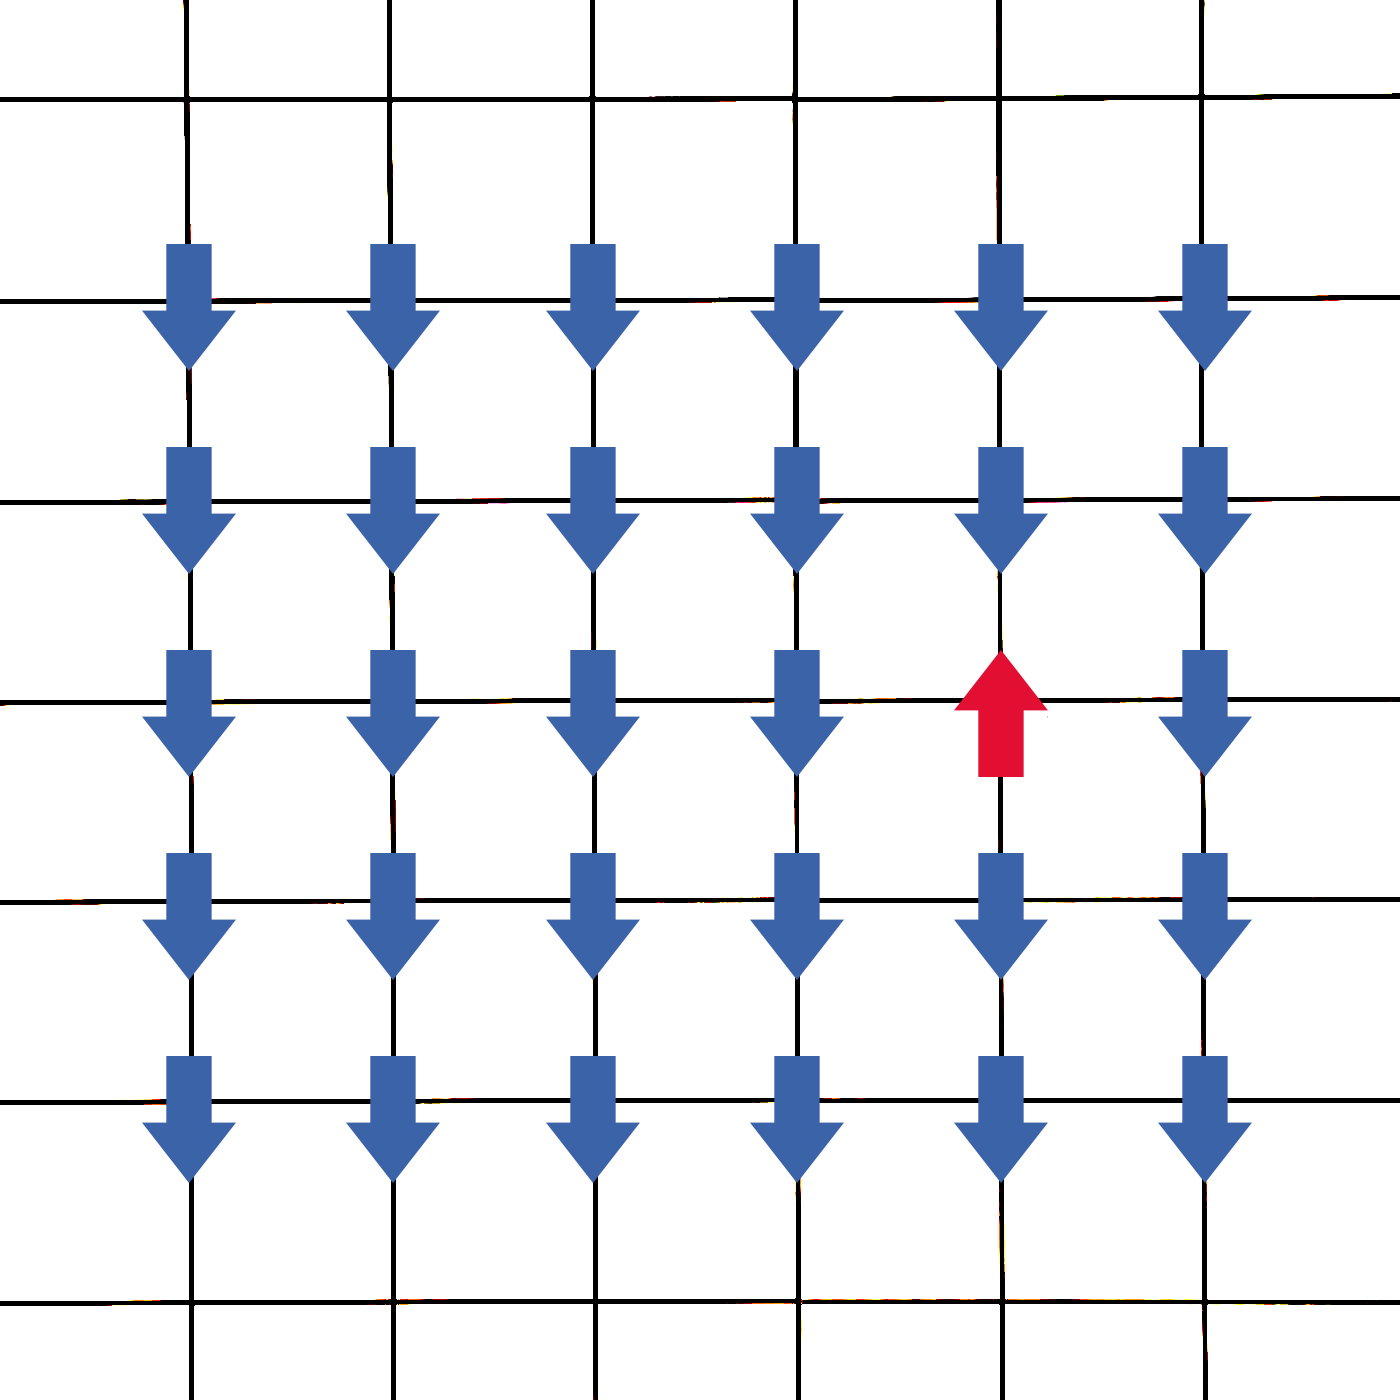
\includegraphics[width=0.4\textwidth]{Immagini/ising.jpg}
\caption{Modello di Ising (EA).}
\label{figura:ising}
\end{wrapfloat}
\cite{QA}Il modello di Ising (IM) a due dimensioni è possibile immaginarlo come una griglia $N \times N$ composta da \textit{nodi}, che rappresentano gli atomi, e \textit{archi}, che rappresentano le interazioni tra essi. Ogni nodo può assumere come valori $1$ in caso l'atomo sia spin-up o $-1$ in caso sia spin-down. Esistono due varianti del modello IM quella di \idx{Sherrington-Kirkpatrick} (SK) dove l'interazione di ogni particella ha raggio infinito e quello di  \idx{Edwards-Anderson} (EA) dove l'interazione ha raggio finito. In questa discussione faremo sempre riferimento al modello EA con raggio unitario, ovvero le particelle interaggiranno soltanto con quelle adiacenti. A questo modello sarà associata una funzione Hamiltoniana:
$$ H(\vec{a}, \vec{b}, \vec{q}) = - \sum_{i \in A } a_i q_i - \frac{1}{2} \sum_{i \in A} \sum_{j \in B_i} b_{ij} q_i q_j $$
in cui $A$ è l'insieme dei nodi e $B_i$ è l'insieme dei vicini del nodo $i$. In particolare $a_i$ è il valore di energia associata al nodo $i$, $q_i$ è il valore dello spin del nodo $i$ e $b_{ij}$ è il valore di energia associato alla coppia di vicinanza dei nodi $i$ e $j$. È importante tenere conto che l'hamiltoniana descritta non fa riferimento al numero di dimensioni, infatti questo modello può essere astratto a $n$ dimensioni.
\lvliii{Algoritmo simulated annealing}
\cite{QA, MC, ST}Il primo step del processo del simulated annealing consiste nel determinare uno stato di
partenza. Solitamente questo avviene in maniera casuale e, perciò, la condizione iniziale può anche essere \textit{non ammissibile}. L’idea alla base dell’algoritmo è quella di arrivare a valutare un sottoinsieme delle soluzioni ammissibili partendo dallo stato iniziale scelto e applicando una successione di piccole perturbazioni.

L'algoritmo prevede un loop di $n$ iterazioni che simula l'abbassamento della temperatura da $t_{max}$ (temperatura di partenza) a $t_{min}$ (temperatura di arrivo) con uno scalino di $t_{delta}$. Dati quindi i parametri iniziali $t_{max}, t_{min} \in \mathbb{R}_{\geq 0}$ e $ t_{delta} \in \mathbb{R}_{> 0}$, possiamo ricavarci il valore di $n$:
$$n = \frac{t_{max}-t_{min}}{t_{delta}}$$
con $n \in \mathbb{N}$ e $t_{max} > t_{min}$.

Ad ogni iterazione del ciclo viene generata una soluzione \textit{vicina} a quella \textit{attuale} e viene deciso quale delle due tenere.

Un esempio di criterio di vicinanza può essere espresso attraverso il peso di Hamming: supponiamo di avere una sequenza di 8 bit $00001111$ con peso di Hamming 4, se noi scegliamo 2 come peso di Hamming massimo di vicinanza, allora una configurazione vicina può essere $00111111$.

Lo step successivo è l'applicazione dal \idx{criterio di Metropolis}, che rappresenta il cuore dell'algoritmo: in questo passo viene scelto se tenere la configurazione \textit{attuale} o la configurazione \textit{vicina}. Se la configurazione \textit{vicina} è migliore di quella \textit{attuale} viene certamente scelta quella \textit{vicina}, contrariamente se quella \textit{attuale} è meglio di quella \textit{vicina} si sceglierà di tenere quella più svantaggiosa delle due (\textit{vicina}) in maniera semi-casuale.
La semi-casualità viene data dalla generazione di un numero casuale $k \in [0,1]$ e dal confrontato con la \idx{distribuzione di Boltzman} di parametri: $t = t_{max} - t_{delta} * n$ e $\Delta E = |E_{vicina}| - |E_{attuale}|$.
$$B(\Delta E, t) = e^{- \frac{\Delta E}{k_B * t}}$$
Questo significa che, in corrispondenza di temperature alte il sistema avrà la possibilità di muoversi liberamente di configurazione in configurazione, mentre all’abbassarsi della temperatura la sua probabilità di accettare soluzioni peggiori diminuirà.

In generale si può vedere l'algoritmo SA come una procedura che mira a minimizzare la configurazione di energia di un sistema dato. Il modello associerà una variabile $\alpha_i \in \mathbb{R}$ modificabile ad ogni costante $\beta_i \in \mathbb{R}$, che rappresenta l'energia per ogni punto del sistema. Intuitivamente si può pensare allo scopo della procedura come quello di trovare gli $\alpha_i$ in modo tale da minimizzare il valore $\alpha_i * \beta_i$. Chiaramente questo è solo un'esempio, la funzione di enegia dipende dal modello di riferimento e quindi può cambiare.

\lvlii{Simulated quantum annealing}
\lvliii{Introduzione}
\cite{QA}L'introduzione del simulated quantum annealing (SQA) avviene per migliorare l'\idx{ergodicità} del sistema, ovvero l'indipendenza della soluzione del problema dallo stato iniziale. Esistono due tipi di ergodicità quella \textit{debole} che delinea una perdita di memoria dello stato iniziale man mano che si evolve il sistema e quella \textit{forte} che prevede la convergenza ad una soluzione indipendentemente dallo stato di partenza. Il SQA migliora l'ergodicità nel caso in cui ci siano due minimi locali divisi da una \idx{spike} (punta di potenziale molto alta e di base stretta) perché la probabilità di transizione da un minimo all'altro è superiore se si sfrutta il \textit{tunneling}(SQA) piuttosto che per \textit{salto} termico(SA).

\lvliii{Modello di Ising trasverso}
\cite{QA}Il modello di Ising trasverso (TIM) nasce per rappresentare l'effetto quantistico che è presente in un insieme di atomi, è possibile immaginarlo come un modello di Ising tradizionale con l'aggiunta di una componente quantistica. Prendiamo di nuovo in esempio il modello di Ising a due dimensioni dove ogni atomo questa volta oltre ad essere in spin-up o spin-down può essere anche in una super position dei due stati. Definiamo quindi un'asse di riferimento ad esempio l'asse x dove andremo alla fine del nostro esperimento a misurare il valore degli spin. Una volta che decideremo di osservare lo stato del sistema nella nostra base x il modello quantistico \textit{collasserà} in quello tradizionale e si comporterà come tale. Oltre alla base di osservazione viene introdotta un'altra base ortogonale alla prima, ad esempio l'asse z, questo asse sarà quello in cui verrà preparato il sistema nella condizione iniziale. L'idea alla base è di far in modo che il modello di Ising passi dalla base z alla base x attraverso uno scheduling da noi scelto. Il coefficente che rappresenta questo scheduling è $\Gamma_{orto}$. L'hemiltoniana del sistema viene così descritta:
$$ H(\vec{a}, \vec{b}, \vec{\sigma}, \vec{\Lambda}, \Gamma_{orto}) = - \sum_{i \in A } a_i \sigma^x_i - \frac{1}{2} \sum_{i \in A} \sum_{j \in B_i} b_{ij} \sigma^x_i \sigma^x_j - \Gamma_{orto} \sum_{i \in A } \Lambda_i \sigma^z_i$$
In questa versione al posto dei valori di spin troviamo le matrici di Pauli $\sigma^x_i$ e $\sigma^z_i$ per rappresentare le super position e in aggiunta dei coefficenti $\Lambda_i$ che parametrizzano l'effetto tunneling.

\lvliii{Approssimazione Suzuki-Trotter}
\begin{wrapfloat}{figure}{I}{0pt}
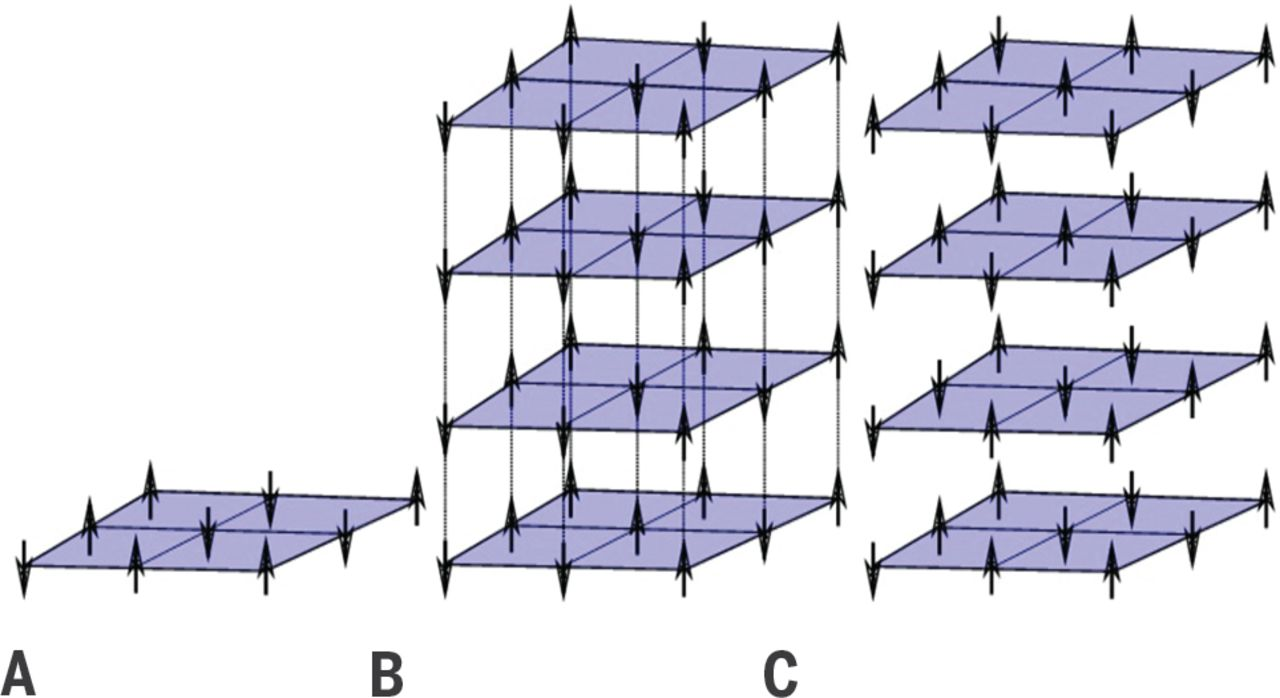
\includegraphics[width=0.4\textwidth]{Immagini/suzuki.jpg}
\caption{Approssimazione Suzuki-Trotter.}
\label{figura:suzuki}
\end{wrapfloat}
\cite{QA, PIMC}Il primo passo per implementare il SQA è approssimare il modello matematico quantistico attraverso un modello classico computabile da un calcolatore tradizionale. Sfruttando il formalismo Suzuki-Trotter possiamo mappare il nostro modello TIM n-dimensionale in un modello IM (n+1)-dimensionale dove la dimensione aggiuntiva rappresenta l'evoluzione temporale del sistema delle sue altre dimensioni. La procedura per ricavarci il modello IM parte dalla considerazione di dividere l'hemiltoniana $H = H_{classic} + H_{kinetic}$ nella sua parte classica di energia potenziale $H_{classic}$ e nella sua parte transversa rappresentante l'energia cinetica $H_{kinetic}$. Ora si può scrivere la \idx{funzione di partizione}
$$Z = Tr (exp(-\frac{H_{classic} + H_{kinetic}}{T}))$$ e attraverso la formula di Trotter riscriverla come:
$$Z= \lim_{M \to +\infty} \sum_i \langle\sigma_i|[exp(-\frac{H_{classic}}{M \cdot T}) \cdot exp(-\frac{H_{kinetic}}{M \cdot T})]^M| \sigma_i\rangle$$
Applicandola alla funzione di partizione possiamo dividere in: la parte potenziale
$$Z_{classic} = \prod^M_{k = 1}\langle\sigma_{1,k}\cdot\cdot\cdot\sigma_{N,k}|exp(\frac{1}{M \cdot T} \sum_{i,j} J_{ij}\sigma^x_i\sigma^x_j)|\sigma_{1,k+1}\cdot\cdot\cdot\sigma_{N,k+1}\rangle = exp(\sum_{i,j=1}^N\sum_{k=1}^M \frac{J_{ij}}{M \cdot T}\sigma_{ik}\sigma_{jk})$$
dove i valori $\sigma_i = \pm 1$ sono gli autovalori dell'operatore $\sigma^x$, e la parte cinetica
$$Z_{kinetic} = \prod^M_{k = 1}\langle\sigma_{1,k}\cdot\cdot\cdot\sigma_{N,k}|exp(\frac{\Gamma}{M \cdot T} \sum_{i}\sigma^z_i)|\sigma_{1,k+1}\cdot\cdot\cdot\sigma_{N,k+1}\rangle =$$
$$= [\frac{1}{2} sinh ( \frac{2\Gamma}{M \cdot T} )]^{\frac{N \cdot M}{2}} exp( \frac{1}{2} ln(coth(\frac{\Gamma}{M \cdot T}))\cdot\sum_{i=1}^N\sum_{k=1}^M \frac{J_{ij}}{M \cdot T}\sigma_{i,k}\sigma_{i,k+1})$$
dove in questo caso $\sigma_i = \pm 1$ sono gli autovalori dell'operatore $\sigma^z$.
A questo punto ricaviamo:
$$ Z \simeq Z_M = C^{NM} \sum_{z^1}\cdot\cdot\cdot\sum_{z^M} exp(\frac{-H_{d+1}}{M\cdot T})$$
ed in fine otteniamo:
$$H_{d+1} = - \sum^M_{k = 1}(\sum_{i,j} J_{i,j} \sigma^k_i \sigma^k_j + J_{orto} \sum_i \sigma^k_i \sigma^{k+1}_i)$$
con  $\sigma_i = \pm 1$ i valori di spin classici, $M$ è la dimensione aggiuntiva, $T$ la temperatura fissa del sistema, $J_{i,j} \in \mathbb{R}$ e
$$J_{orto} = - \frac{M\cdot T}{2} ln(tanh(\frac{\Gamma}{M \cdot T}))$$
$H_{d+1}$ rappresenta l'energia associata alla funzione di partizione $Z_M$ che è assintotica a $Z$ per un sistema alla temperatura $M \cdot T$.

\lvliii{Algoritmo Santoro-Tosatti-Martonak}
L'algoritmo chiamto \textit{Santoro-Tosatti-Martonak} o anche come \textit{Path Integral Monte Carlo} (PIMC)\cite{PIMC} è un'algorimto che cerca di ottenere il valore minimo di energia per IM attraverso a delle modifiche locali nella discrettizzazione della dinamica di evoluzione degli spin nel tempo.

Come prima cosa si sceglie un valore $M$ che rappresenta il numero di approssimazione nella dimensione temporale.
Successivamente si inizializza IM in equilibrio ad una temperatura $T$, lo si duplica $M$ volte e lo si interconnette creando un modello TIM impostando un valore di $J_{orto} \simeq T \cdot M \cdot K(t) \ge |J|$ dove $K(t)$ è una funzione da determinare e $J$ è il valore di accoppiamento degli spin. Un modo per portare il modello IM in equilibrio è partire da una configurazione casuale e successivamente applicare un SA da $T_{iniz}$ a $T$ con $T_{iniz} > T$.
Il valore $K(t) = -ln(tanh(\frac{\Gamma}{M \cdot T}))$ viene determinato scegliendo una $\Gamma_{max}$ iniziale. Un buon modo per sceglierla è fare delle simulazioni brevi preventive per testare alcuni valori $\Gamma_{max}$ scelti arbitrariamente. Il valore deve essere non troppo alto altrimenti non ci sarà l'accoppiamento nella dimensione temporale e neppure troppo basso se no l'accoppiamentro sarà troppo alto e l'algoritmo avrà le stesse prestazioni di quello classico.

L'algoritmo prevede un loop di $n$ iterazioni denominate \textit{Monte Carlo Step} (\idx{MCS}) che simulano il collassamento da superposition ad osservabile diminuendo l'inverso della correlazione da $\Gamma_{max}$ (particelle scorrelate) a $\Gamma_{min}$ (particelle correlate) con uno scalino di $\Gamma_{delta}$.
Vengono definite due tipi di mosse: quella locale dove si inverte uno spin e quella globale dove si inverte un'intera colonna di spin nell'asse temporale.
Durante ogni MCS vengono eseguite sia una mossa globale che una locale con criterio di accettazione uguale a quello del SA (criterio di Metropolis) considerando l'energia del TIM al posto del IM.

L'algoritmo si conclude selezionando il modello IM con energia minore all'interno del TIM.

\lvliii{Algoritmo CT-SQA}
Il \textit{continuos time simulated quantum annealing} (CT-SQA)\cite{QVC} anche chiamato \textit{Riger-Kawashima}\cite{CTSQA} è una variante del Monte Carlo a cluster \textit{Swendsen-Wang}\cite{NCD} ed è un'algorimto che cerca di ottenere il valore minimo di energia per IM attraverso a delle modifiche non locali di raggruppamenti in cluset dei segmenti continui nella dinamica di evoluzione degli spin nel tempo.

Ancora una volta per applicare un algoritmo quantistico in uno tradizionale bisogna approssimare il modello TIM n-dimensionale in un modello IM (n+1)-dimensionale attraverso l'approssimazione Suzuki-Trotter con condizioni al contorno periodiche; ottenendo la solita funzione classica di energia:
$$S_{class} = - \sum_{\tau,\langle ij \rangle} K_{ij} S_i(\tau) S_j(\tau) - \sum_{\tau, i} K_{i}' S_i(\tau) S_i(\tau+1)$$
che questa volta viene utilizzata per esprimere l'energia libera del sistema:
$$F = - T \cdot \lim_{\Delta \tau \to 0} \ln(Tr(e^{-S_{class}}))$$
dove la forza di intrazione tra gli spin di fette temporali consecutivi è
$$K_{i}' = - \frac{1}{2} ln( tanh( \Delta \tau \Gamma_i) )$$
mentre la forza di interazione degli spin sulla stessa fetta temporale è
$$K_{ij} = \Delta \tau J_{ij}$$
Il numero di fette temporali $L_{\tau}$ è legato a $\Delta \tau = \frac{1}{T \cdot L_{\tau}}$ in modo che $\Delta \tau \to 0$ implica $L_{\tau} \to \infty$.
Per ottenere un algoritmo continuo ci interessa quindi avere un numero infinito di fette che equivale a dire $\Delta \tau \to 0$, ma essendo computazionalmente improponibile viene scelto di tenere $L_{\tau} \coloneqq M$ limitato considerando spin paralleli e adiacenti in intervalli temporali differenti, come \idx{segmenti} temporali limitati agli estremi dai \idx{cut} che li dividono da altri segmenti aventi lo spin nell'altro verso.

Prima di vedere l'algoritmo introduciamo le probabilità neccessarie al suo funzionamento iniziando dalle probabilità di due spin adiacenti di avere lo stesso verso a seconda se abbiano un legame temporale o spaziale:
la probabilità di due spin spazio-adiacenti di avere lo stesso verso è
$$p_{ij} = 1 - e^{-2K_{ij}} = 2\Delta \tau J_{ij} + o(\Delta \tau^2)$$
mentre la probabilità di due spin tempo-adiacenti di avere lo stesso verso è
$$p_i' = 1 - e^{-2K_{i}'} = 1 - \Delta \Gamma_{i} + o(\Delta \tau^2)$$
Queste probabilità vengono utilizzate attraverso l'algoritmo Monte Carlo per introdurre altri cut.
Da qui si può esprimere la probabilità di un certo spin $i$ di collegarsi al suo tempo-adiacente in un segmento di lunghezza $t < \beta$:
$$\tilde{p_i} = \lim_{\Delta \tau \to 0} p_i'^{\frac{t}{\Delta \tau}} = \lim_{\Delta \tau \to 0} (1 - \Delta \tau \Gamma_i)^\frac{t}{\Delta \tau} = e^{- \Gamma_i t}$$
che servirà all'algoritmo per introdurre nuovi cut con probabilità
$$p_{cut}(i) = 1 - \tilde{p_i}$$
con probabilità che diminuisce col diminuire della lunghezza.
Con lo stesso ragionamento di può anche dedurre la probabilità di un certo spin $ij$ di non collegare due segmenti $S_i\{[t_1, t_2]\}$ e $S_j\{[t_3, t_4]\}$:
$$\tilde{p_{ij}} = \lim_{\Delta \tau \to 0} (1 - p_{ij})^\frac{t}{\Delta \tau} = \lim_{\Delta \tau \to 0} (1 - 2\Delta \tau J_{ij})^\frac{t}{\Delta \tau} = e^{-2 t J_{ij}}$$
con $t$ la lunghezza dell'intervallo $[t_1, t_2] \cap [t_3, t_4]$; che servirà all'algoritmo per collegare due segmenti creando un \idx{cluster} con probabilità
$$p_{join}(i,j) = 1 - \tilde{p_{i,j}}$$

L'algoritmo prevede gli stessi passaggi del \textit{Santoro-Tosatti-Martonak} a differenza della procedura eseguita all'interno del MCS che verrà spiegata qui sotto.
Per ogni spin vengono generati dei tagli tra le sue repliche temporali con probabilità  di taglio $p_{cut}(i)$.
Successivamente per ogni spin e per ogni sua evoluzione temporale si esegue un tentativo di unione a cluster con probabilità $p_{join}(i,j)$.
A questo punto per ogni cluster verrà eseguita un'inversione di spin con probabilità $p_{flip} = 0.5$, verranno quindi memorizzate le energie delle fette temporali, verranno rimossi i tagli superflui contenuti nei segmenti continui e rimossi i join.

\lvliii{Algoritmo DT-SQA}
Come il CT-SQA ma con le probabilità non calcolate per $\Delta \tau \to 0$.
